\documentclass{beamer}
\usepackage{natbib}

\begin{document}
\title{Simultaneous Treatment of Random and Systematic Errors in the Historical Radiosonde Temperature Archive}
\author{Josh Browning}
\date{\today} 

\frame{\titlepage} 

\frame{\frametitle{Table of contents}\tableofcontents} 

\section{Problem}

\frame{
\frametitle{Project Overview}
\textbf{Problem:} Random and systematic errors exist in the radiosonde temperature archive, and no studies have addressed how to handle both types of errors simultaneously.\\
\textbf{Proposed Solution:}  I propose studying the effect of applying various sequences of quality control algorithms on simulated data which is designed to have the same structure as true radiosonde data.
}	

\subsection{Radiosonde Data}
\frame{
\frametitle{Radiosonde Data}
\begin{columns}
	\begin{column}{.3\textwidth}
		\begin{figure}
			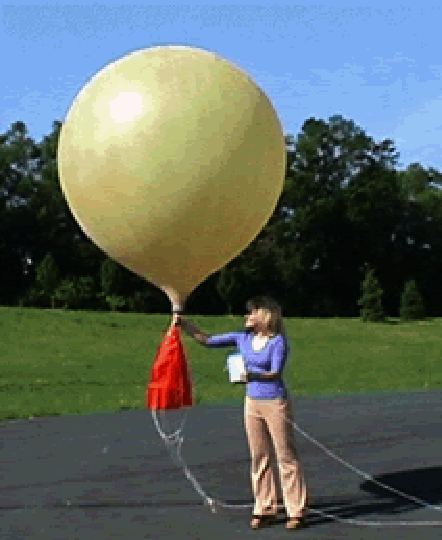
\includegraphics[width=.7\textwidth]{radiosonde_launch-eps-converted-to.pdf}
			\caption{Sample Radiosonde}
			\label{fig:radio}
		\end{figure}
		\begin{figure}
			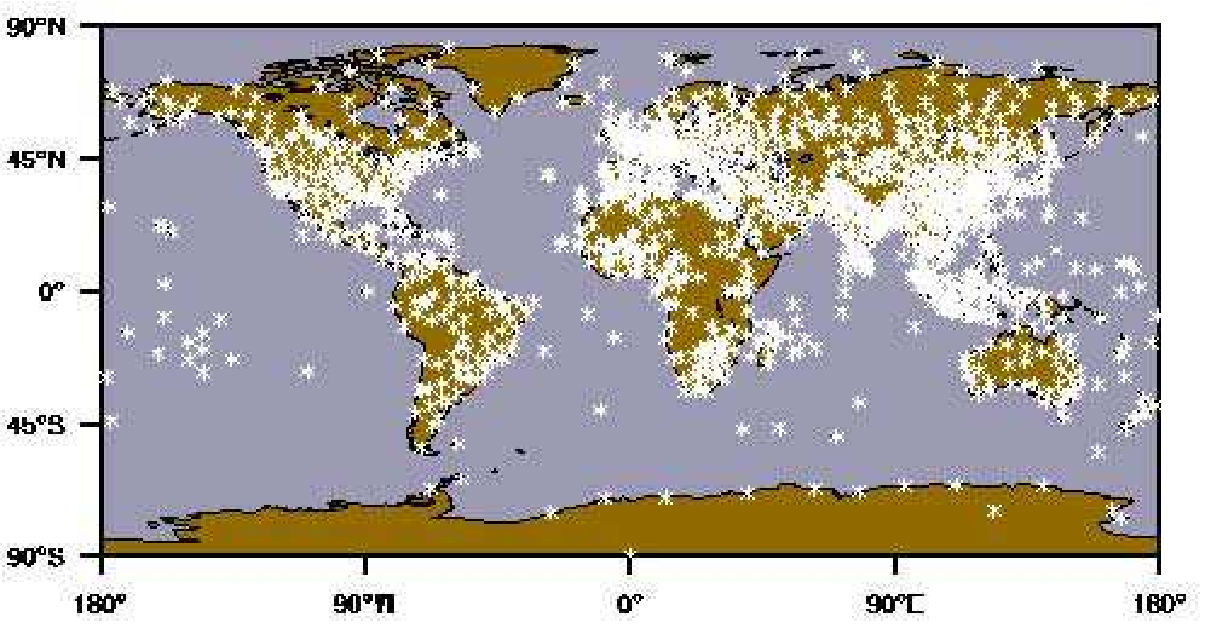
\includegraphics[width=\textwidth]{GlobalRadiosondeNetwork2-eps-converted-to.pdf}
			\caption{Global Radiosonde Network}
			\label{fig:global}
		\end{figure}
	\end{column}
	\begin{column}{.7\textwidth}
		\begin{itemize}
			\item Small instruments are suspended below 2m hydrogen or helium balloons.
			\item They measure atmospheric variables such as temperature, wind speed, etc.
			\item Balloons are launched twice daily at roughly 00 UTC and 12 UTC, and at 700 sites worldwide.
			\item More than 1,300 additional launch sites exist in the historical archive.
			\item Considering the number of launch sites, multiple observations for different pressure levels, and the total number of launches, there are between 50 and 90 million historical soundings.
		\end{itemize}
	\end{column}
\end{columns}
}

\subsection{Random Errors}

\frame{\frametitle{Problems with the data: Random Errors}
	\begin{columns}
		\begin{column}{.4\textwidth}
			Random errors can occur because of
			\begin{enumerate}
				\item Faulty data transmission
				\item Sporadic instrumentation problems
				\item Keystroke entries
				\item Errors in data management
				\item Many other reasons
			\end{enumerate}
		\end{column}
		\begin{column}{.6\textwidth}
			\begin{figure}
				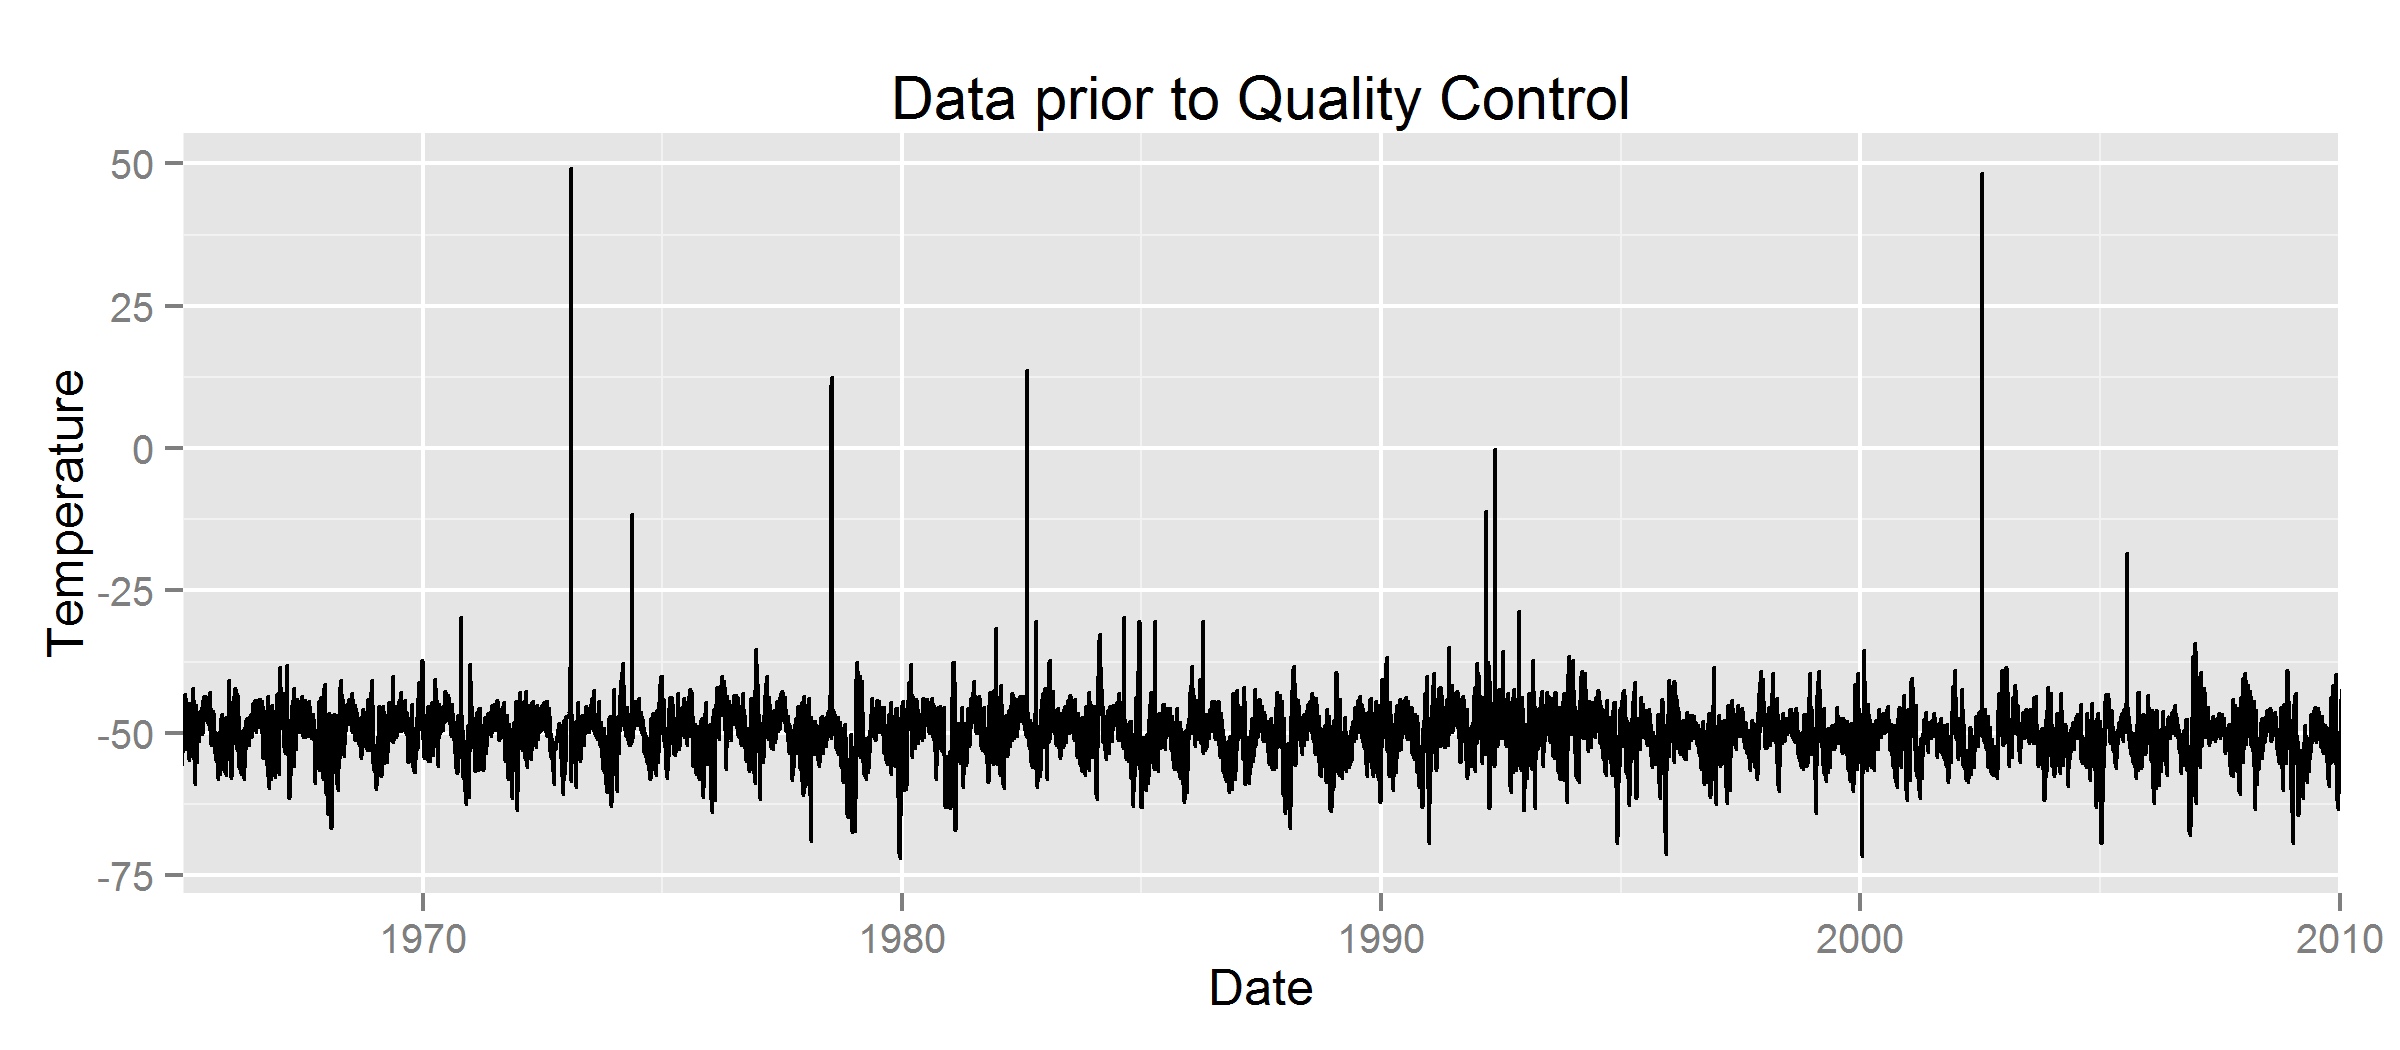
\includegraphics[width=\textwidth]{70219_Data_Unhomogenized_no_vlines}
				\label{fig:70219_out}
				\caption{Data collected from Station 70219 in Bethel, Alaska.}
			\end{figure}
		\end{column}
	\end{columns}
}

\subsection{Systematic Errors}
\frame{\frametitle{Problems with the data: Systematic Errors}
	\begin{columns}
		\begin{column}{.4\textwidth}
			Systematic errors can occur because of
			\begin{enumerate}
				\item Station location changes
				\item Urbanization of the area surrounding the station
				\item Changes in instrumentation
				\item Many other reasons
			\end{enumerate}
		\end{column}
		\begin{column}{.6\textwidth}
			\begin{figure}
				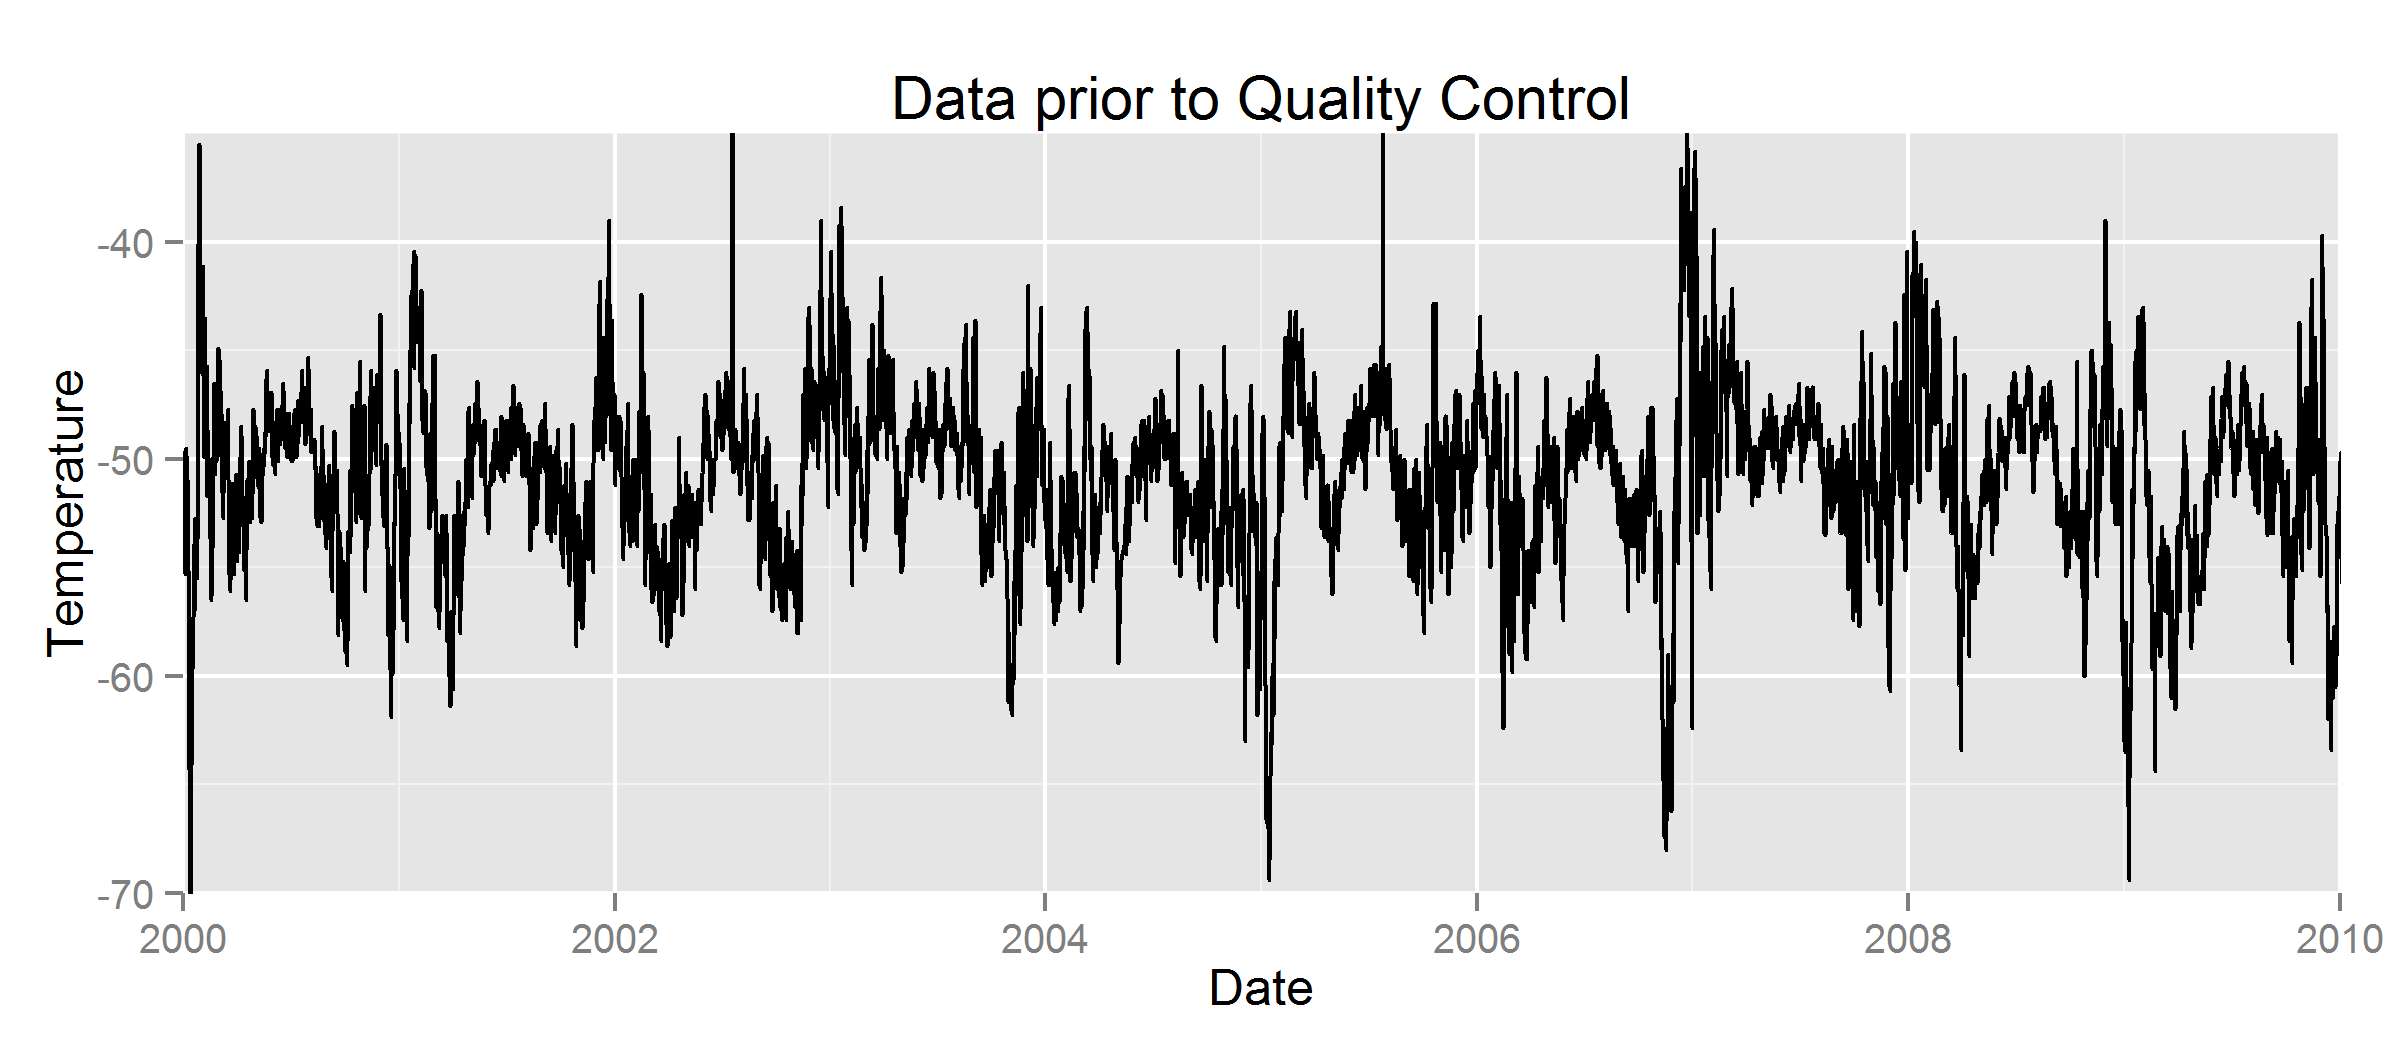
\includegraphics[width=\textwidth]{70219_Data_Unhomogenized_zoomed_no_vlines}
				\label{fig:70219_in}
				\caption{Data collected from Station 70219 in Bethel, Alaska.}
			\end{figure}
		\end{column}
	\end{columns}
}

\section{Methods}

\subsection{Random Error Detection}
\frame{\frametitle{Random Error Detection Methods}
	\begin{itemize}
		\item The simplest way to detect random errors is to estimate the mean and standard deviation of the data and then to label observations as random errors if they are more than $k$ standard deviations from the mean (where $k$ may be 5 or so).
		\item In \cite{bell14}, a better alternative is proposed which uses robust estimates of the mean and standard deviation (more details on next slide).
		\item I propose using these techniques in my simulation study.
	\end{itemize}
}

\frame{\frametitle{More on Robust Mean and Standard Deviation}
\footnotesize
\begin{enumerate}
	\item First, the estimates of the mean, $\hat{\mu}$, and standard deviation, $\hat{\sigma}$, are initialized to
	\begin{align*}
	\hat{\mu} &= \mbox{median}(\mathbf{x})\\
	\hat{\sigma} &= \mbox{MAD}(\mathbf{x}),
	\end{align*}
	where $\mathbf{x}$ is a vector of the data, and $MAD$ is the median absolute deviation, defined as
	\begin{equation*}
	MAD = \mbox{median}( \lvert x_i - \mbox{median}(\mathbf{x}) \rvert ).
	\end{equation*}
	\item Then, Winsorized values, $y_i$, are computed.  These are defined as
	\begin{equation*}
	y_i = \left\{ \begin{array}{ll}
	\hat{\mu}-k \hat{\sigma} & : x_i \leq \hat{\mu}-k \hat{\sigma}\\
	x_i & : \hat{\mu}-k \hat{\sigma} < x_i \leq \hat{\mu}+k \hat{\sigma}\\
	\hat{\mu}+k \hat{\sigma} & : x_i > \hat{\mu}+k \hat{\sigma}\\
	\end{array} \right.
	\end{equation*}
	\item Updated estimates of $\hat{\mu}$ and $\hat{\sigma}$ are computed as the mean of $\mathbf{y}$ and the standard deviation of $\mathbf{y}$, respectively.
	\item Steps 2 and 3 are repeated until $\hat{\mu}$ changes by less than $10^{-6} \hat{\sigma}$.
\end{enumerate}
Note: In step 3, one may choose to estimate $\hat{\sigma}_L$ and $\hat{\sigma}_R$ using only observations to the left and right, respectively, of the mean.  This allows for improved outlier detection with skewed data.
}

\subsection{Systematic Error Correction (Homogenization)}
\frame{\frametitle{Systematic Error Correction (Homogenization)}
	\begin{itemize}
		\item Many homogenization methods have been proposed in the climate literature: \cite{eskridge95, haimberger07, lanzante96, lanzante03, venema12}.  However, these methods are not generally robust to outliers.
		\item Modern homogenization methods are also presented in the statistical literature \cite{killick12, scott74}.
		\item I propose comparing these methods and developing a homogenization method that is robust to outliers.
	\end{itemize}
}

\frame{\frametitle{Homogenization Methods: SNHT}
	\small
	This algorithm is commonly used in the climate literature.  The algorithm works as follows:
	\begin{enumerate}
		\item For each observation, two means are computed: one for the $N$ days prior to observation $i$, $\bar{X}_{L,i}$, and one for the $N$ days following, $\bar{X}_{R,i}$
		\item Then, the test statistic
			\begin{equation}
			T_i = \frac{N}{s_i}\left( (\bar{X}_{L,i}-\bar{X}_i)^2 + (\bar{X}_{R,i}-\bar{X}_i)^2\right),
			\label{eq:Hom}
			\end{equation}
		is computed where $\bar{X}_i$ is the mean of $\bar{X}_{L,i}$ and $\bar{X}_{R,i}$, and $s_i$ is the estimated standard deviation over the $N$ days prior and $N$ days following observation $i$.  \item If the largest $T_i$ exceeds some threshold at time $i=i^*$, I conclude that a change point occurred at time $i^*$, and I adjust all observations after time $i^*$ by $\bar{X}_{L,i^*}-\bar{X}_{R,i^*}$.  A threshold of 100 is recommended in \cite{haimberger07}.
		\item Repeat steps 1-3 until no test statistic exceeds the threshold.
	\end{enumerate}
}

\frame{\frametitle{Homogenization Methods: Robust SNHT}
	\begin{itemize}
		\item The previous algorithm is not robust to random errors, as the influence function for the sample mean is unbounded.
		\item The Winsorized estimator of center and scale discussed previously is robust against random errors.
		\item Thus, to create a robust SNHT statistic, I propose replacing the means and standard deviation in Equation~(\ref{eq:Hom}) with these estimators.
	\end{itemize}
}

\frame{\frametitle{Homogenization Methods: BinSeg}
\begin{itemize}
	\item Several homogenization methods work by optimizing a cost function:
	\begin{equation}
	\sum_{i=1}^{m+1} [\mathcal{C}(y_{(\tau_{i-1}+1):\tau_i})] + \beta f(m),
	\label{eq:cost}
	\end{equation}
	where $\tau_i$ is the $i$th change point; $m$ is the number of change points; $\mathcal{C}$ is a cost function; $y_{(\tau_{i-1}+1):\tau_i}$ is the observed data between the $(i-1)$ and $i$th change point; and $\beta f(m)$ is a penalty term on the number of change points, see \cite{killick12}.
	\item Often, $\mathcal{C}$ is chosen to be twice the negative log likelihood, and $f(\cdot)$ is linear.
	\item Binary Segmentation (BinSeg) uses a greedy algorithm: at each step, a changepoint is selected which minimizes the cost function.  The data is then partitioned in two, and optimization continues iteratively.
\end{itemize}
}

\frame{\frametitle{Homogenization Methods: PELT}
\begin{itemize}
	\item Pruned Exact Linear Time (PELT) is another algorithm for optimizing Equation (\ref{eq:cost}), but it computes the exact minimum.
	\item It proceeds recursively as follows: first, the optimal number and location of change points is determined for observations 1 and 2 only.  The optimal number and location of change points for the first three observations is then determined using this information, and more generally the optimal number and location of change points for the first $k+1$ observations is determined by considering the optimal configurations for the first $2, 3, \ldots, k$ observations.
	\item PELT is computationally efficient, and is implemented in the \texttt{changepoint} package in R \cite{killick14}.
\end{itemize}
}

\subsection{Sequencing}
\frame{\frametitle{Quality Control Algorithm Sequencing}
	\begin{itemize}
		\item I am also interested in understanding the effect that the sequence of the quality control algorithms has on the overall quality control procedure.
		\item Let ``Ran'' denote the random error detection algorithm and ``Sys'' the systematic error correction algorithm.  Then, I propose investigating the following alternatives:
		\begin{itemize}
			\item Ran$\to$Sys
			\item Sys$\to$Ran
			\item Ran$\to$Sys$\to$Ran
			\item Sys$\to$Ran$\to$Sys
		\end{itemize}
	\end{itemize}
}

\section{Simulation Design}
\frame{\frametitle{Overall Simulation Design}
	To understand the effect of these various algorithms/sequencings on the final quality controlled dataset, I propose the following simulation design:
	\begin{enumerate}
		\item Using observed radiosonde data, develop a data generating mechanism with which to simulate data from.
		\item Simulate a dataset using the model from step 1, and contaminate it with systematic and random errors.
		\item Apply the quality control algorithms described above to the simulated dataset, and determine
		\begin{itemize}
			\item The best homogenization algorithms for sub-daily data in the presence of random errors
			\item The best sequencing in the presence of both random and systematic errors
		\end{itemize}
		\item Repeat steps 2 and 3 1,000 times for each of 10 different radiosonde stations and 3 pressure levels.
	\end{enumerate}
}

\subsection{Modeling Data}

\frame{\frametitle{Modeling Radiosonde Data- Part 1}
\begin{enumerate}
	\item In order to capture seasonal and hourly trends, I plan on fitting a Generalized Additive Model (GAM) to the radiosonde temperature data.
	\item GAMs are flexible, non-parametric models that allow the response variable to be a linear combination of smoothed functions of the input variables, see \cite{hastie90}.
	\item The particular model I'll fit is
	\begin{equation} \label{eq:GAM}
		t_i = \beta_0 + s_1(h_i) + s_2(d_i) + \beta_1 y_i + \epsilon_i,
	\end{equation}
	where $t_i$ is the temperature at a given station and pressure level; $h_i$, $d_i$ and $y_i$ are the hour, day, and year of the $i$-th observation, respectively; $\beta_0$ is the intercept; $\beta_1$ is the coefficient for the long term trend; and $s_1(\cdot)$ and $s_2(\cdot)$ are cubic regression splines.
\end{enumerate}  
}

\frame{\frametitle{Modeling Radiosonde Data- Part 2}
\begin{enumerate}
	\item Typically the error term, $\epsilon_i$, in the GAM model would be modeled as normal with some unknown variance, but the distribution of the error terms could be skewed or have heavier tails than a normal distribution.
	\item Thus, I'll use a skew-$t$ distribution for the errors of this model, which has 4 parameters, $\xi, \sigma, \alpha$, and $\nu$ which are useful in controlling the first four moments of the distribution, see \cite{azzalini03}.
\end{enumerate}
}

\frame{\frametitle{Modeling Radiosonde Data- Part 3}
\begin{enumerate}
	\small
	\item Additionally, I expect there to be temporal correlation in the error terms.
	\item Since I have already included hourly and seasonal terms in the model, I expect most of this autocorrelation to be explained, and so an AR(1) time series model is sufficient to account for the remaining structure in the residuals.
	\item For radiosonde data, observations are not equally spaced in time:  Launches are scheduled globally at 0 and 12 UTC, but many deviations from this pattern are observed.
	\item Thus, to estimate the lag-$h$  autocorrelation, ${\phi}(h)$, in hours, I must use only those observations that are $h$ time steps apart:
	\begin{equation} \label{eq:ACF}
	\widehat{\phi}(h)=\frac{1}{\lvert \mathcal{P}_h\rvert} \sum_{(\widehat{\epsilon_i},\widehat{\epsilon_j}) \in \mathcal{P}_h} \frac{(\widehat{\epsilon_i}-\bar{\epsilon_i})(\widehat{\epsilon_j}-\bar{\epsilon_j})}{\sqrt{s_{\epsilon_i} s_{\epsilon_j}}},
	\end{equation}
	where $\mathcal{P}_h$ is the set of all pairs of residuals that are $h$ hours apart (or within some window), and $\widehat{\epsilon_i}$ is the observed residual from Equation~(\ref{eq:GAM}).
	\item For an AR(1) model, I need only estimate $\phi(\cdot)$ at $h=12$ hours, and I plan on using a window of 5\% of 12 hours, or 0.6 hours.
\end{enumerate}
}

\subsection{Performance Metrics}

\frame{\frametitle{Performance Metrics}
	\small
	\begin{itemize}
		\item \textbf{True Positive Rate:}  The proportion of simulated errors correctly detected by the quality control algorithm.
		\item \textbf{False Positive Rate:}  The proportion of valid data points incorrectly identified as errors by the quality control algorithm.
		\item \textbf{Efficiency:}  Let $\mathbf{x}$, $\mathbf{c}$, and $\mathbf{h}$ be the original, contaminated, and contaminated and homogenized time series, respectively and let the $i$-th observation be denoted by $x_i, c_i$, and $h_i$ respectively.  The Root Mean Square Error (RMSE) of $\mathbf{h}$ is then defined as follows:
		\begin{equation*}
		\mbox{RMSE}(\mathbf{h}) = \sqrt{\frac{1}{n} \sum_{i=1}^n (h_i-x_i)^2}.
		\end{equation*}
		Then, the efficiency of the homogenized series, where 1 means perfect skill, 0 means no improvement, and negative values indicate degradation is
		\begin{equation*}
		\mbox{Eff}(\mathbf{h}) = \frac{\mbox{RMSE}(\mathbf{c})-\mbox{RMSE}(\mathbf{h})}{\mbox{RMSE}(\mathbf{c})}.
		\end{equation*}
	\end{itemize}
}

\frame{\frametitle{Summary of Proposed Study}
	For the defense, a summary of the simulation study will be given along with conclusions on the performance of the various homogenization algorithms and sequencings.  Additionally, the recommended method will be applied to an actual dataset as a case study.
}

\section{References}

\frame[shrink=30]{\frametitle{References}
	\footnotesize
	\bibliographystyle{myabbrvnat}
	\bibliography{mybib}
}


\end{document}